
%(BEGIN_QUESTION)
% Copyright 2011, Tony R. Kuphaldt, released under the Creative Commons Attribution License (v 1.0)
% This means you may do almost anything with this work of mine, so long as you give me proper credit

An operator tells you the stack temperature of this incinerator is running high as indicated by TIC-37.  The setpoint is set at 1400 degrees F, but the PV display shows a steady 1489 $^{o}$F:

$$\includegraphics[width=15.5cm]{i0004rx01.eps}$$

Identify the likelihood of each specified fault in this process.  Consider each fault one at a time (i.e. no coincidental faults), determining whether or not each fault could independently account for {\it all} measurements and symptoms in this process.

% No blank lines allowed between lines of an \halign structure!
% I use comments (%) instead, so that TeX doesn't choke.

$$\vbox{\offinterlineskip
\halign{\strut
\vrule \quad\hfil # \ \hfil & 
\vrule \quad\hfil # \ \hfil & 
\vrule \quad\hfil # \ \hfil \vrule \cr
\noalign{\hrule}
%
% First row
{\bf Fault} & {\bf Possible} & {\bf Impossible} \cr
%
\noalign{\hrule}
%
% Another row
TT-37 miscalibrated (reading too low) &  &  \cr
%
\noalign{\hrule}
%
% Another row
TT-37 miscalibrated (reading too high) &  &  \cr
%
\noalign{\hrule}
%
% Another row
TIC-37 in manual mode &  &  \cr
%
\noalign{\hrule}
%
% Another row
TIC-37 in auto mode &  &  \cr
%
\noalign{\hrule}
%
% Another row
FIC-38 in manual mode &  &  \cr
%
\noalign{\hrule}
%
% Another row
FIC-38 in auto mode &  &  \cr
%
\noalign{\hrule}
%
% Another row
FIC-38 in cascade mode &  &  \cr
%
\noalign{\hrule}
%
% Another row
FT-38 miscalibrated (reading too low) &  &  \cr
%
\noalign{\hrule}
} % End of \halign 
}$$ % End of \vbox

\underbar{file i03529}
%(END_QUESTION)





%(BEGIN_ANSWER)

% No blank lines allowed between lines of an \halign structure!
% I use comments (%) instead, so that TeX doesn't choke.

$$\vbox{\offinterlineskip
\halign{\strut
\vrule \quad\hfil # \ \hfil & 
\vrule \quad\hfil # \ \hfil & 
\vrule \quad\hfil # \ \hfil \vrule \cr
\noalign{\hrule}
%
% First row
{\bf Fault} & {\bf Possible} & {\bf Impossible} \cr
%
\noalign{\hrule}
%
% Another row
TT-37 miscalibrated (reading too low) &  & $\surd$ \cr
%
\noalign{\hrule}
%
% Another row
TT-37 miscalibrated (reading too high) &  & $\surd$ \cr
%
\noalign{\hrule}
%
% Another row
TIC-37 in manual mode & $\surd$ &  \cr
%
\noalign{\hrule}
%
% Another row
TIC-37 in auto mode &  & $\surd$ \cr
%
\noalign{\hrule}
%
% Another row
FIC-38 in manual mode & $\surd$ &  \cr
%
\noalign{\hrule}
%
% Another row
FIC-38 in auto mode & $\surd$ &  \cr
%
\noalign{\hrule}
%
% Another row
FIC-38 in cascade mode &  & $\surd$ \cr
%
\noalign{\hrule}
%
% Another row
FT-38 miscalibrated (reading too low) &  & $\surd$ \cr
%
\noalign{\hrule}
} % End of \halign 
}$$ % End of \vbox


%(END_ANSWER)





%(BEGIN_NOTES)

\filbreak \vskip 20pt \vbox{\hrule \hbox{\strut \vrule{} {\bf Virtual Troubleshooting} \vrule} \hrule}

\noindent
{\bf Predicting the effect of a given fault:} present each of the following faults to the students, one at a time, having them comment on all the effects each fault would produce.

\begin{itemize}
\item{} 
\item{} 
\item{} 
\end{itemize}


\vskip 10pt


\noindent
{\bf Identifying possible/impossible faults:} present symptoms to the students and then have them determine whether or not a series of suggested faults could account for all the symptoms, explaining {\it why} or {\it why not} for each proposed fault:

\begin{itemize}
\item{} Symptom: {\it TAL-36 is alarming, with TIC-37 showing an abnormally low temperature and its output at 100\%}
\item{} TT-37 failed with low signal -- {\bf No}
\item{} TT-37 failed with high signal -- {\bf No}
\item{} FIC-38 in ``Auto'' mode rather than ``Cascade'' mode -- {\bf Yes}
\item{} FIC-38 in ``Manual'' mode rather than ``Cascade'' mode -- {\bf Yes}
\item{} Open fault in wiring to SV-115 -- {\bf Yes}
\item{} TIC-37 in ``Manual'' mode rather than ``Auto'' mode -- {\bf Yes}
\item{} FT-38 failed with low signal -- {\bf No}
\item{} FT-38 failed with high signal -- {\bf Yes}
\end{itemize}


\vskip 10pt


\noindent
{\bf Determining the utility of given diagnostic tests:} present symptoms to the students and then propose the following diagnostic tests one by one.  Students rate the value of each test, determining whether or not it would give useful information (i.e. tell us something we don't already know).  Students determine what different results for each test would indicate about the fault, if anything:

\begin{itemize}
\item{} Symptom: {\it }
\item{}  -- {\bf Yes/No}
\item{}  -- {\bf Yes/No}
\end{itemize}


\vskip 10pt


\noindent
{\bf Diagnosing a fault based on given symptoms:} imagine the TT-37 is miscalibrated such that it reads 250 $^{o}$F too high (don't reveal the fault to students!).  Present the operator's observation(s) to the students, have them consider possible faults and diagnostic strategies, and then tell them the results of tests they propose based on the following symptoms, until they have properly identified the nature and location of the fault:

\begin{itemize}
\item{} Operator observation: {\it Analyzers are registering excessive H$_{2}$S emissions, and also noting that TIR-36 reads about 250 degrees F below setpoint}
\item{} TIC-37 SP = 1500 $^{o}$F
\item{} TIC-37 PV = 1495 $^{o}$F
\item{} TIC-37 Out = 35\%
\item{} FIC-38 SP = 35\%
\item{} FIC-38 PV = 35\%
\item{} FIC-38 Out = 23\%
\item{} BMS shows normal operation (proven flame)
\end{itemize}


%INDEX% Basics, control loop troubleshooting (realistic P&ID shown)
%INDEX% Control, strategies: cascade (realistic P&ID shown)
%INDEX% Fieldbus, HART: multivariable instrument (realistic P&ID shown)
%INDEX% Process: incinerator (realistic P&ID shown)

%(END_NOTES)

